\documentclass[a4paper,10pt]{article}
\usepackage[margin=1in]{geometry}
\usepackage{amsmath}
\usepackage{pgfplots}
\usepackage{amsfonts}
\usepackage{multirow}
\usepackage{graphicx}
\usepackage{caption}
\usepackage{subcaption}
\usepackage{grffile}
\begin{document}
\title{Report}
\maketitle
\section*{Evaluation Data}
16
 
				\begin{table}[htbp]
				\centering
				\begin{tabular}{|c|c|c|c|}
				\hline
				algorithm&precision&recall&fscore\\
				\hline
				textblocksBS.py&0.25615801016&0.633801236527&0.342120282718\\
VerticalDominance0.py&0.215106607996&0.499821978044&0.289447986537\\
VerticalDominance1.py&0.544540452936&0.52399888488&0.519786884455\\

				\hline
				\end{tabular}
				\end{table}
				 
\section*{Performance Curve}
\begin{figure}[!htbp]
\centering
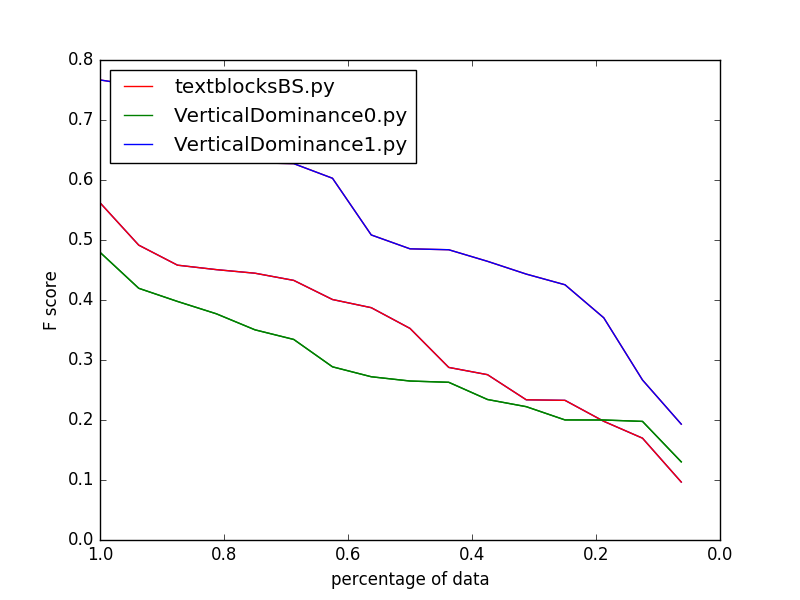
\includegraphics[width = 15cm]{performance.png} 
\end{figure}
\section*{Outliers}
\subsection*{Good outliers}
filter: 0.7
 
				\begin{table}[htbp]
				\centering
				\begin{tabular}{|c|c|c|}
				\hline
				filename&algorithm&score\\
				\hline
				0003.jpg&VerticalDominance1.py&0.766761768902\\
0005.jpg&VerticalDominance1.py&0.756710451171\\

				\hline
				\end{tabular}
				\end{table}
				 
\subsection*{Bad outliers}
filter: 0.4
 
				\begin{table}[htbp]
				\centering
				\begin{tabular}{|c|c|c|}
				\hline
				filename&algorithm&score\\
				\hline
				0006.jpg&textblocksBS.py&0.287642276423\\
0034.jpg&textblocksBS.py&0.275540275049\\
0035.jpg&textblocksBS.py&0.197841726619\\
0037.jpg&textblocksBS.py&0.0965804066543\\
0038.jpg&textblocksBS.py&0.169708029197\\
0045.jpg&textblocksBS.py&0.387198986058\\
0259.jpg&textblocksBS.py&0.232761726349\\
0292.jpg&textblocksBS.py&0.352644836272\\
0296.jpg&textblocksBS.py&0.233676975945\\
0003.jpg&VerticalDominance0.py&0.377064756615\\
0006.jpg&VerticalDominance0.py&0.288625592417\\
0033.jpg&VerticalDominance0.py&0.397590361446\\
0034.jpg&VerticalDominance0.py&0.350291639663\\
0035.jpg&VerticalDominance0.py&0.222222222222\\
0036.jpg&VerticalDominance0.py&0.334257547751\\
0037.jpg&VerticalDominance0.py&0.2\\
0038.jpg&VerticalDominance0.py&0.264957264957\\
0045.jpg&VerticalDominance0.py&0.272090777402\\
0253.jpg&VerticalDominance0.py&0.197667087011\\
0255.jpg&VerticalDominance0.py&0.23416391474\\
0259.jpg&VerticalDominance0.py&0.262838657501\\
0292.jpg&VerticalDominance0.py&0.13023255814\\
0296.jpg&VerticalDominance0.py&0.200114025086\\
0035.jpg&VerticalDominance1.py&0.37037037037\\
0037.jpg&VerticalDominance1.py&0.266666666667\\
0292.jpg&VerticalDominance1.py&0.193103448276\\

				\hline
				\end{tabular}
				\end{table}
				 
\newpage
	
					\begin{figure}
					\centering
					\begin{subfigure}{.5\textwidth}
					  \centering
					  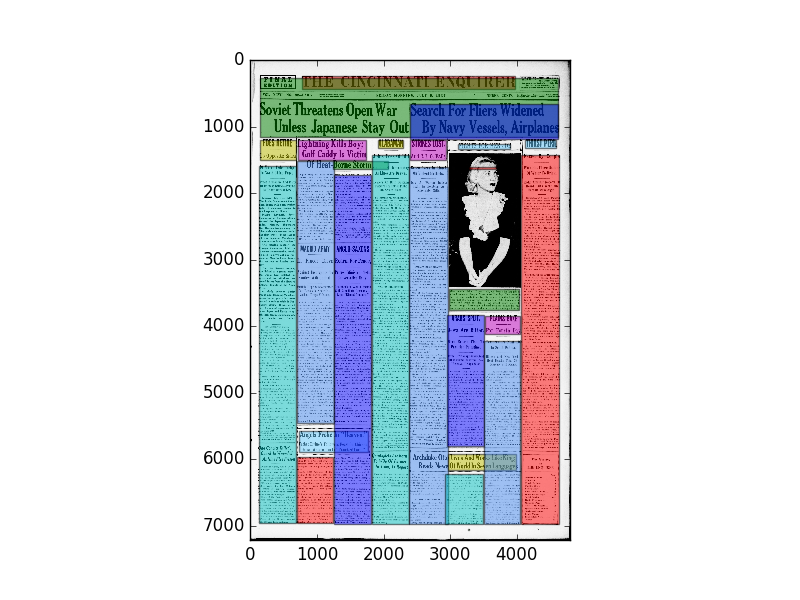
\includegraphics[width=10cm]
					{textblocksBS.py.best.png}
					  \caption{best result}
					  \label{fig:sub1}
					\end{subfigure}%
					\begin{subfigure}{.5\textwidth}
					  \centering
					  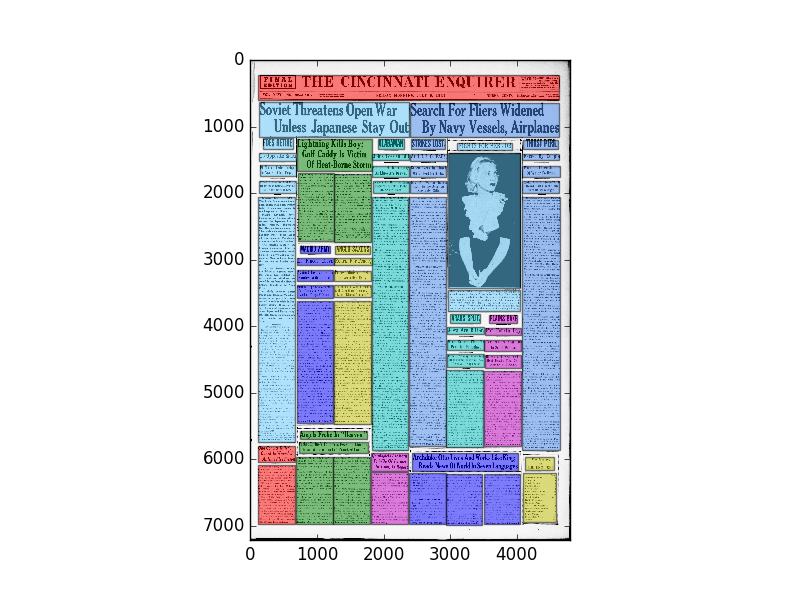
\includegraphics[width=10cm]
					{textblocksBS.py.gt.best.png}
					  \caption{ground truth}
					  \label{fig:sub2}
					\end{subfigure}
					\caption
					{best result of textblocksBS.py}
					\label{fig:test}
					\end{figure}
						
					\begin{figure}
					\centering
					\begin{subfigure}{.5\textwidth}
					  \centering
					  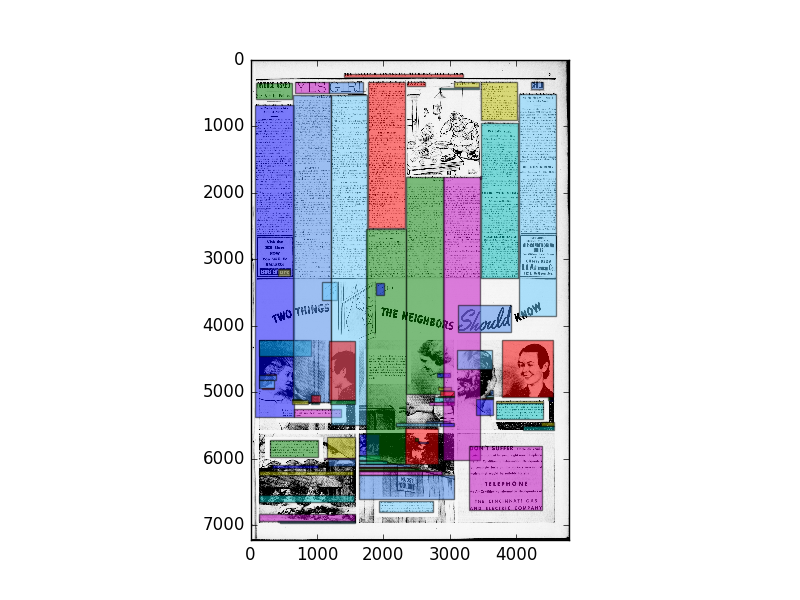
\includegraphics[width=10cm]
					{textblocksBS.py.worst.png}
					  \caption{worst result}
					  \label{fig:sub1}
					\end{subfigure}%
					\begin{subfigure}{.5\textwidth}
					  \centering
					  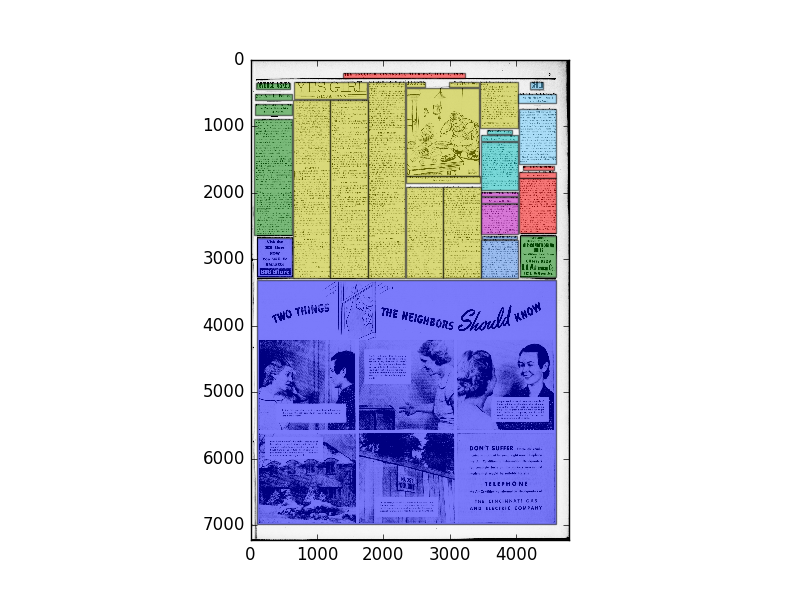
\includegraphics[width=10cm]
					{textblocksBS.py.gt.worst.png}
					  \caption{ground truth}
					  \label{fig:sub2}
					\end{subfigure}
					\caption
					{worst result of textblocksBS.py}
					\label{fig:test}
					\end{figure}
						
					\begin{figure}
					\centering
					\begin{subfigure}{.5\textwidth}
					  \centering
					  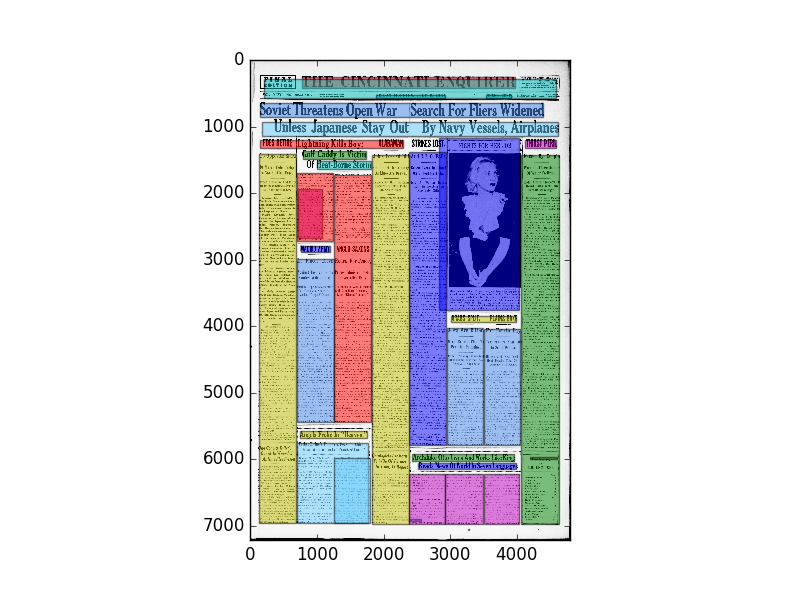
\includegraphics[width=10cm]
					{VerticalDominance0.py.best.png}
					  \caption{best result}
					  \label{fig:sub1}
					\end{subfigure}%
					\begin{subfigure}{.5\textwidth}
					  \centering
					  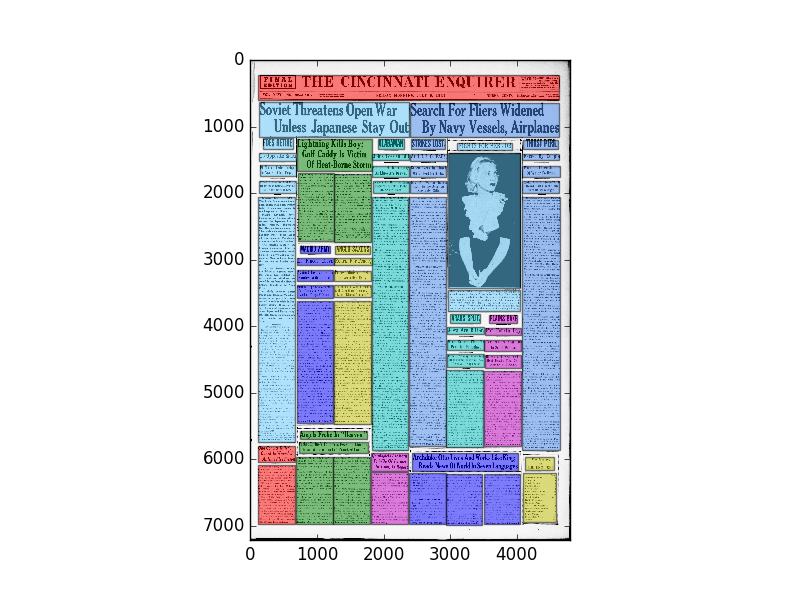
\includegraphics[width=10cm]
					{VerticalDominance0.py.gt.best.png}
					  \caption{ground truth}
					  \label{fig:sub2}
					\end{subfigure}
					\caption
					{best result of VerticalDominance0.py}
					\label{fig:test}
					\end{figure}
						
					\begin{figure}
					\centering
					\begin{subfigure}{.5\textwidth}
					  \centering
					  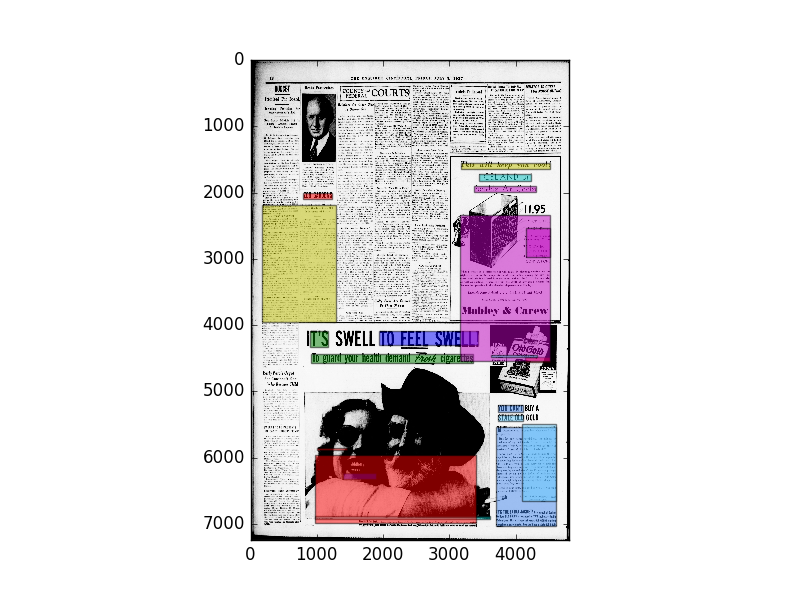
\includegraphics[width=10cm]
					{VerticalDominance0.py.worst.png}
					  \caption{worst result}
					  \label{fig:sub1}
					\end{subfigure}%
					\begin{subfigure}{.5\textwidth}
					  \centering
					  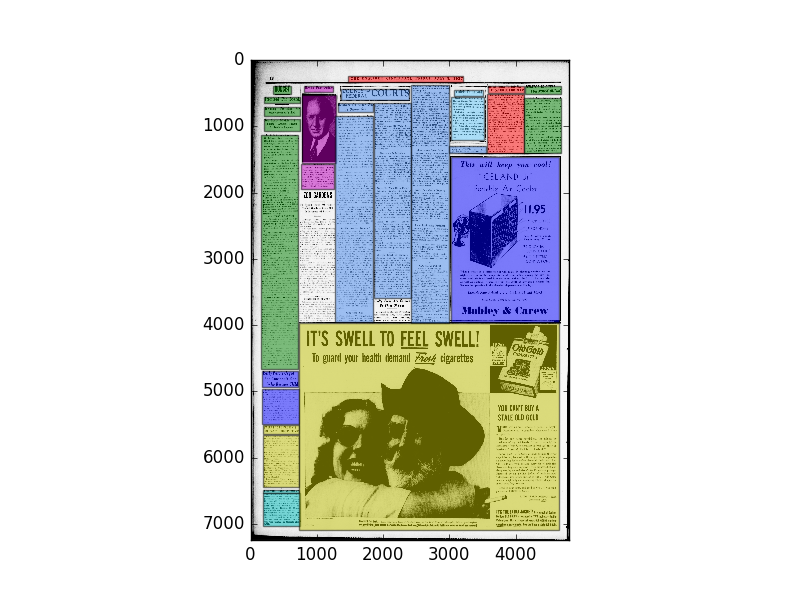
\includegraphics[width=10cm]
					{VerticalDominance0.py.gt.worst.png}
					  \caption{ground truth}
					  \label{fig:sub2}
					\end{subfigure}
					\caption
					{worst result of VerticalDominance0.py}
					\label{fig:test}
					\end{figure}
						
					\begin{figure}
					\centering
					\begin{subfigure}{.5\textwidth}
					  \centering
					  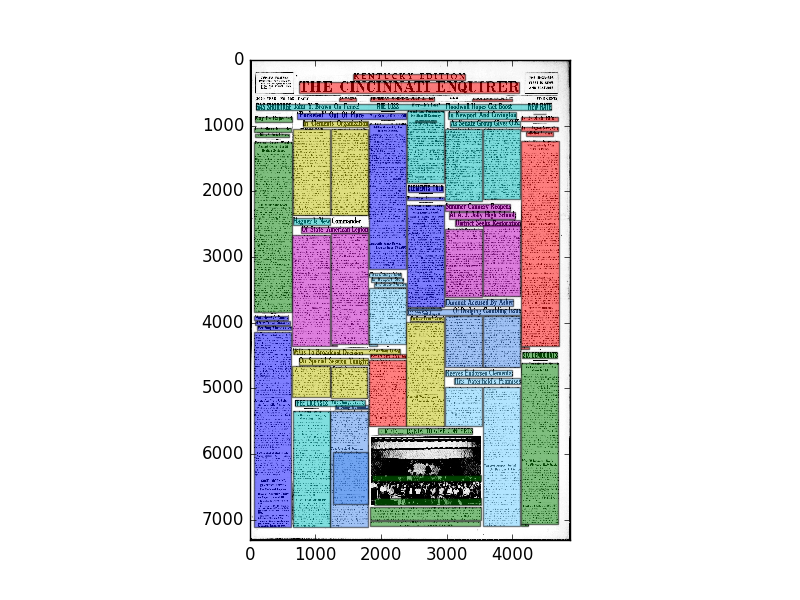
\includegraphics[width=10cm]
					{VerticalDominance1.py.best.png}
					  \caption{best result}
					  \label{fig:sub1}
					\end{subfigure}%
					\begin{subfigure}{.5\textwidth}
					  \centering
					  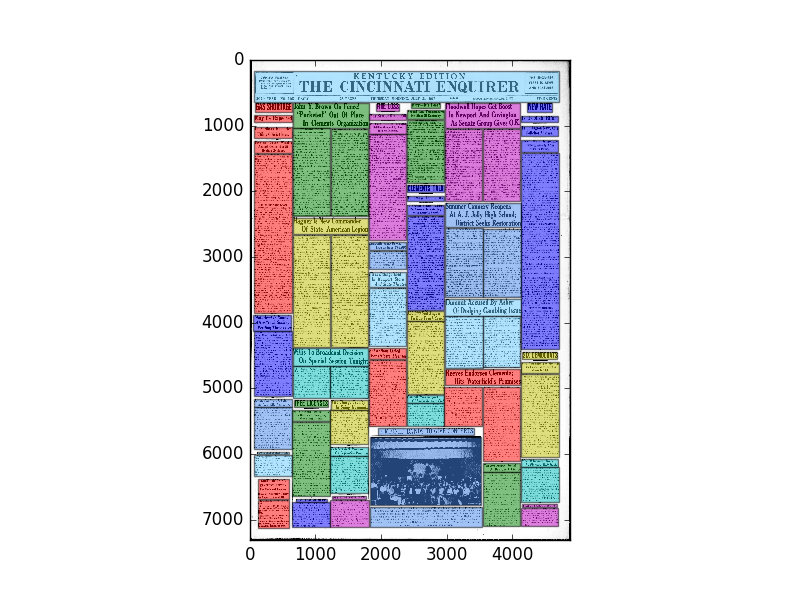
\includegraphics[width=10cm]
					{VerticalDominance1.py.gt.best.png}
					  \caption{ground truth}
					  \label{fig:sub2}
					\end{subfigure}
					\caption
					{best result of VerticalDominance1.py}
					\label{fig:test}
					\end{figure}
						
					\begin{figure}
					\centering
					\begin{subfigure}{.5\textwidth}
					  \centering
					  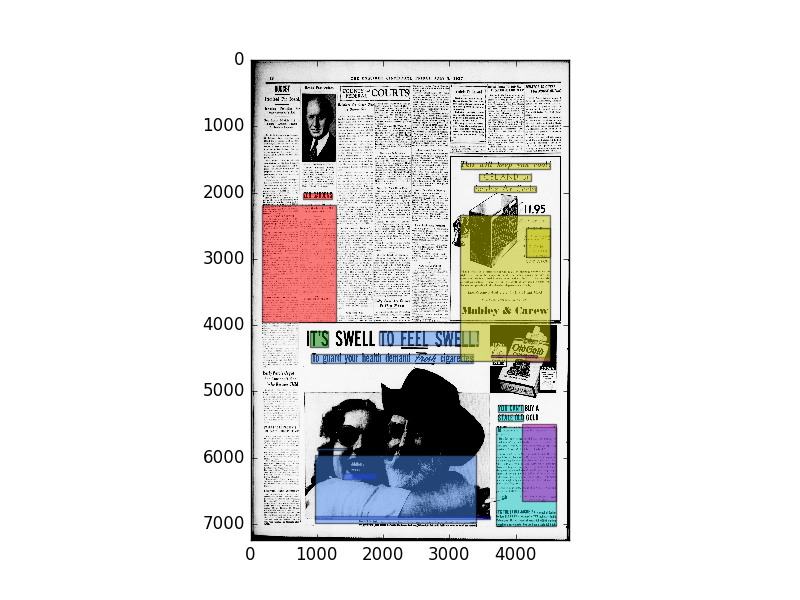
\includegraphics[width=10cm]
					{VerticalDominance1.py.worst.png}
					  \caption{worst result}
					  \label{fig:sub1}
					\end{subfigure}%
					\begin{subfigure}{.5\textwidth}
					  \centering
					  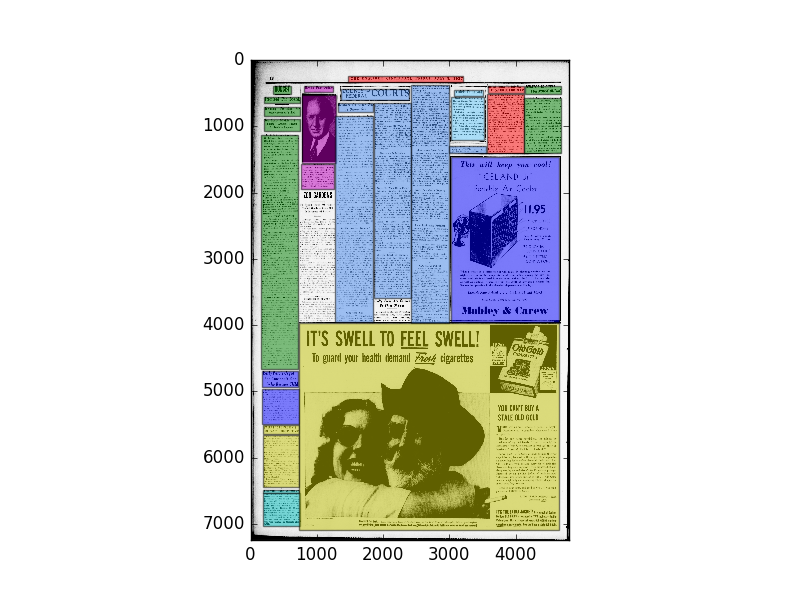
\includegraphics[width=10cm]
					{VerticalDominance1.py.gt.worst.png}
					  \caption{ground truth}
					  \label{fig:sub2}
					\end{subfigure}
					\caption
					{worst result of VerticalDominance1.py}
					\label{fig:test}
					\end{figure}
					
\end{document}